%Preamble
\documentclass[12pt]{article}
\usepackage{fancyhdr}
\usepackage{extramarks}
\usepackage{amsmath}
\usepackage{amssymb}
\usepackage{amsthm}
\usepackage{amsrefs}
\usepackage{amsfonts}
\usepackage{mathrsfs}
\usepackage{mathtools}
\usepackage[mathcal]{eucal} %% changes meaning of \mathcal
\usepackage{enumerate}
\usepackage[shortlabels]{enumitem}
\usepackage{verbatim} %% includes comment environment
\usepackage{hyperref}
\usepackage[capitalize]{cleveref}
\crefformat{equation}{~(#2#1#3)}
\usepackage{caption, subcaption}
\usepackage{graphicx}
\usepackage{fullpage} %%smaller margins
\usepackage[all,arc]{xy}
\usepackage{mathrsfs}

\hypersetup{
    linktoc=all,     % set to all if you want both sections and subsections linked
}

\topmargin=-0.45in
\evensidemargin=0in
\oddsidemargin=0in
\textwidth=6.5in
\textheight=9.0in
\headsep=0.25in
\setlength{\headheight}{16pt}

\linespread{1.0}

\pagestyle{fancy}
\lhead{\Name}
\chead{\hwClass: \hwTitle}
\rhead{\hwDueDate}
\lfoot{\lastxmark}
\cfoot{\thepage}

\renewcommand\headrulewidth{0.4pt}
\renewcommand\footrulewidth{0.4pt}

\setlength\parindent{0pt}

%% Title Info
\newcommand{\hwTitle}{HW \# 7}
\newcommand{\hwDueDate}{March 12, 2021}
\newcommand{\hwClass}{AMATH 568}
\newcommand{\hwClassTime}{}
\newcommand{\hwClassInstructor}{}
\newcommand{\Name}{\textbf{Marlin Figgins}}


%% MATH MACROS
\newcommand{\bbF}{\mathbb{F}}
\newcommand{\bbN}{\mathbb{N}}
\newcommand{\bbQ}{\mathbb{Q}}
\newcommand{\bbR}{\mathbb{R}}
\newcommand{\bbZ}{\mathbb{Z}}
\newcommand{\bbC}{\mathbb{C}}
\newcommand{\abs}[1]{ \left| #1 \right| }
\newcommand{\diff}[2]{\frac{d #1}{d #2}}
\newcommand{\infsum}[1]{\sum_{#1}^{\infty}}
\newcommand{\norm}[1]{ \left|\left| #1 \right|\right| }
\newcommand{\eval}[1]{ \left. #1 \right| }
\newcommand{\Expect}[1]{\mathbb{E}\left[#1 \right]}
\newcommand{\Var}[1]{\mathbb{V}\left[#1 \right]}
\renewcommand{\vec}[1]{\mathbf{#1}}

\renewcommand{\phi}{\varphi}
\renewcommand{\emptyset}{\O}

%--------Theorem Environments--------
%theoremstyle{plain} --- defaultx
\newtheorem{thm}{Theorem}[section]
\newtheorem{cor}[thm]{Corollary}
\newtheorem{prop}[thm]{Proposition}
\newtheorem{lem}[thm]{Lemma}
\newtheorem{conj}[thm]{Conjecture}
\newtheorem{quest}[thm]{Question}

\theoremstyle{definition}
\newtheorem{defn}[thm]{Definition}
\newtheorem{defns}[thm]{Definitions}
\newtheorem{con}[thm]{Construction}
\newtheorem{exmp}[thm]{Example}
\newtheorem{exmps}[thm]{Examples}
\newtheorem{notn}[thm]{Notation}
\newtheorem{notns}[thm]{Notations}
\newtheorem{addm}[thm]{Addendum}

% Environments for answers and solutions
\newtheorem{exer}{Exercise}
\newtheorem{sol}{Solution}

\theoremstyle{remark}
\newtheorem{rem}[thm]{Remark}
\newtheorem{rems}[thm]{Remarks}
\newtheorem{warn}[thm]{Warning}
\newtheorem{sch}[thm]{Scholium}

\makeatletter
\let\c@equation\c@thm
\makeatother

\begin{document}

\begin{exer}

Consider the inverted pendulum dynamics
\begin{equation*}
    u'' + (\delta + \epsilon \cos \omega t) \sin u = 0.
\end{equation*}
\begin{enumerate}[(a)]
    \item Perform a Floquet analysis (computationally) of the pendulum with continous forceing $\cos \omega t$ 
    \item Evaluate for what values of $\delta$, $\epsilon$, and $\omega$ the pendulum is stabilized.
\end{enumerate}
\end{exer}

\begin{sol}
    a) We perform a Floquet analysis computationally by simulating the ODE above with two sets of intial conditions
    \begin{align*}
        u_{1}(0) = 0, u_{1}'(0) = 1\\
        u_{2}(0) = 1, u_{2}'(0) = 0.
    \end{align*}
    We can then compute the Floquet discriminant as
    \begin{align*}
        \Gamma = u_{1}(T) + u_{2}'(T),
    \end{align*}
    where $T = 2\pi / \omega$. Notice that since we can vary the parameters in the ODE, $\Gamma$ is can be viewed as a function of $(\delta, \epsilon, \omega)$. We also recreate figure 36 from the class notes using the given equation. That is, we visualize $\Gamma$ as a function of $\omega$ for two regimes of  $\delta$ and  $\epsilon$ which are  $\delta > \epsilon$ and  $\delta < \epsilon$. This is shown in Figure \ref{fig:floquet-omega}. We observe that for large values of $\omega$, $\Gamma$ approaches 2 in both regimes. Suggesting that the pendulum is stabilized under high frequency forcing.

    b) We also generate heatmaps for $\Gamma$ for fixed $\omega$ and varying $\delta$ and $\epsilon$ to see for which values the solution is stable i.e. 
    \begin{align*}
    \abs{\Gamma(\delta, \epsilon, \omega)} < 2. 
    \end{align*}
    These heatmaps can be seen in Figure \ref{fig:floquet-heat}. We find that for large enoough of $\omega$ nearly all solutions are stable regardless of the choice of $\delta, \epsilon$. 

    \begin{figure}[b]
        \centering
        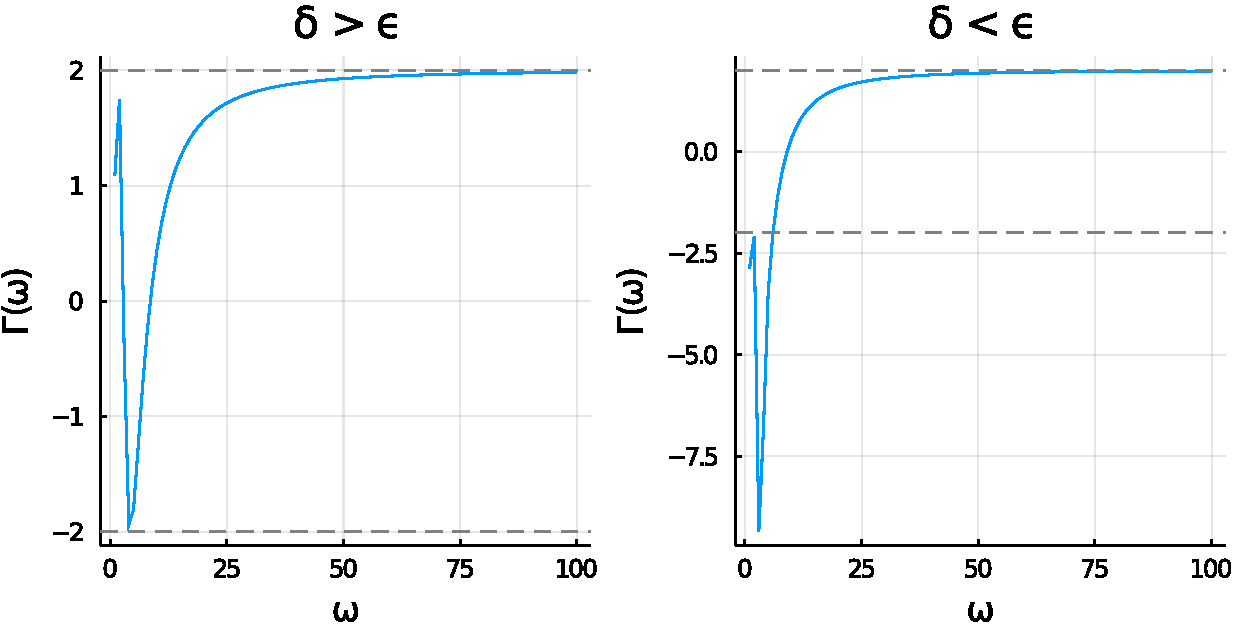
\includegraphics[width=0.8\linewidth]{figs/hw-7-exer-Floquet-omega.pdf}
        \caption{We visualize the Floquet discriminant as a function of $\omega$ in two parameter regimes.}%
        \label{fig:floquet-omega}
    \end{figure}

    \begin{figure}[b]
     \centering
     \begin{subfigure}{\linewidth}
         \centering
         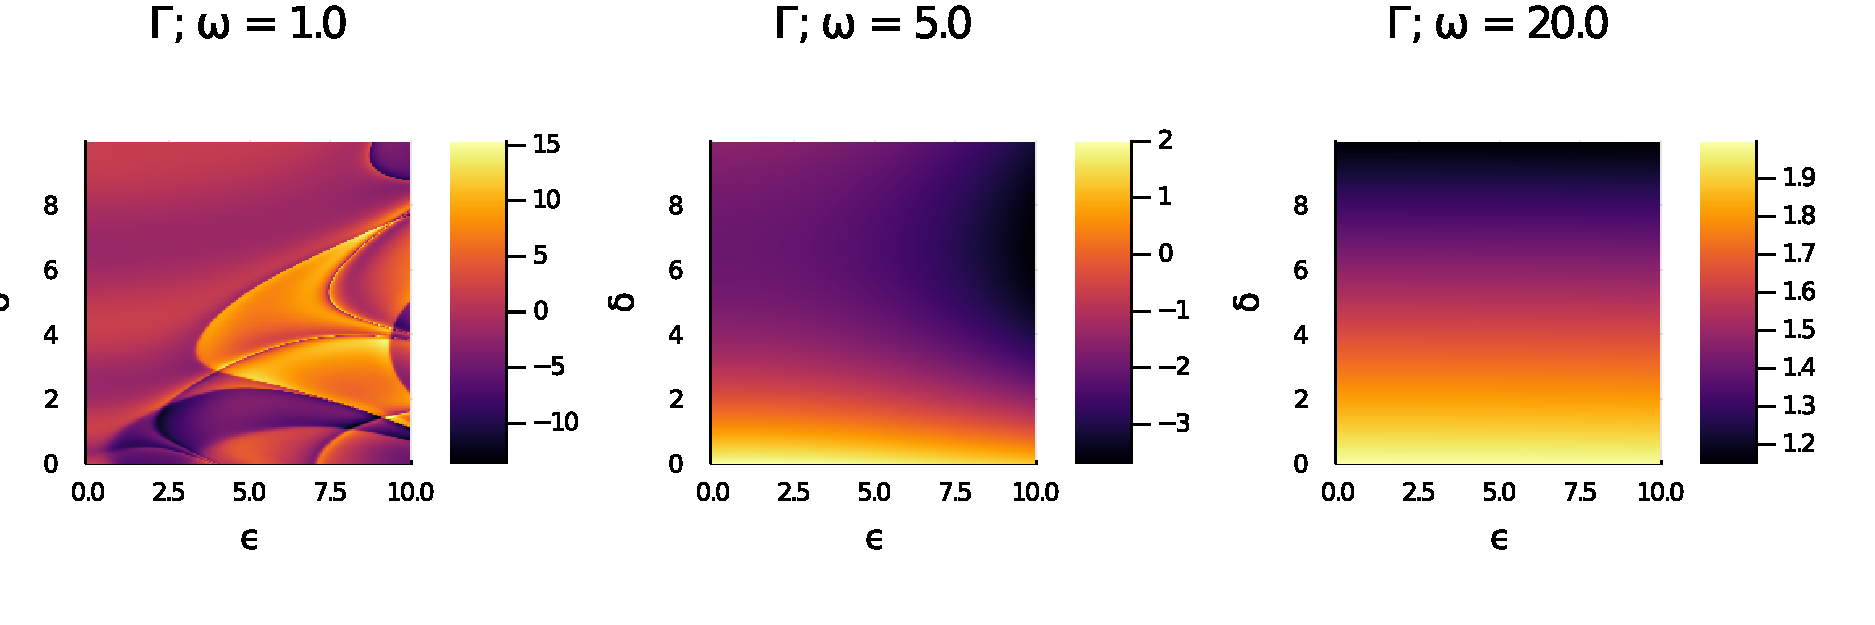
\includegraphics[width=0.9\textwidth]{../hw/figs/hw-7-exer-Floquet-heatmap.pdf}
     \end{subfigure}
     \hfill
     \begin{subfigure}{\linewidth}
         \centering
         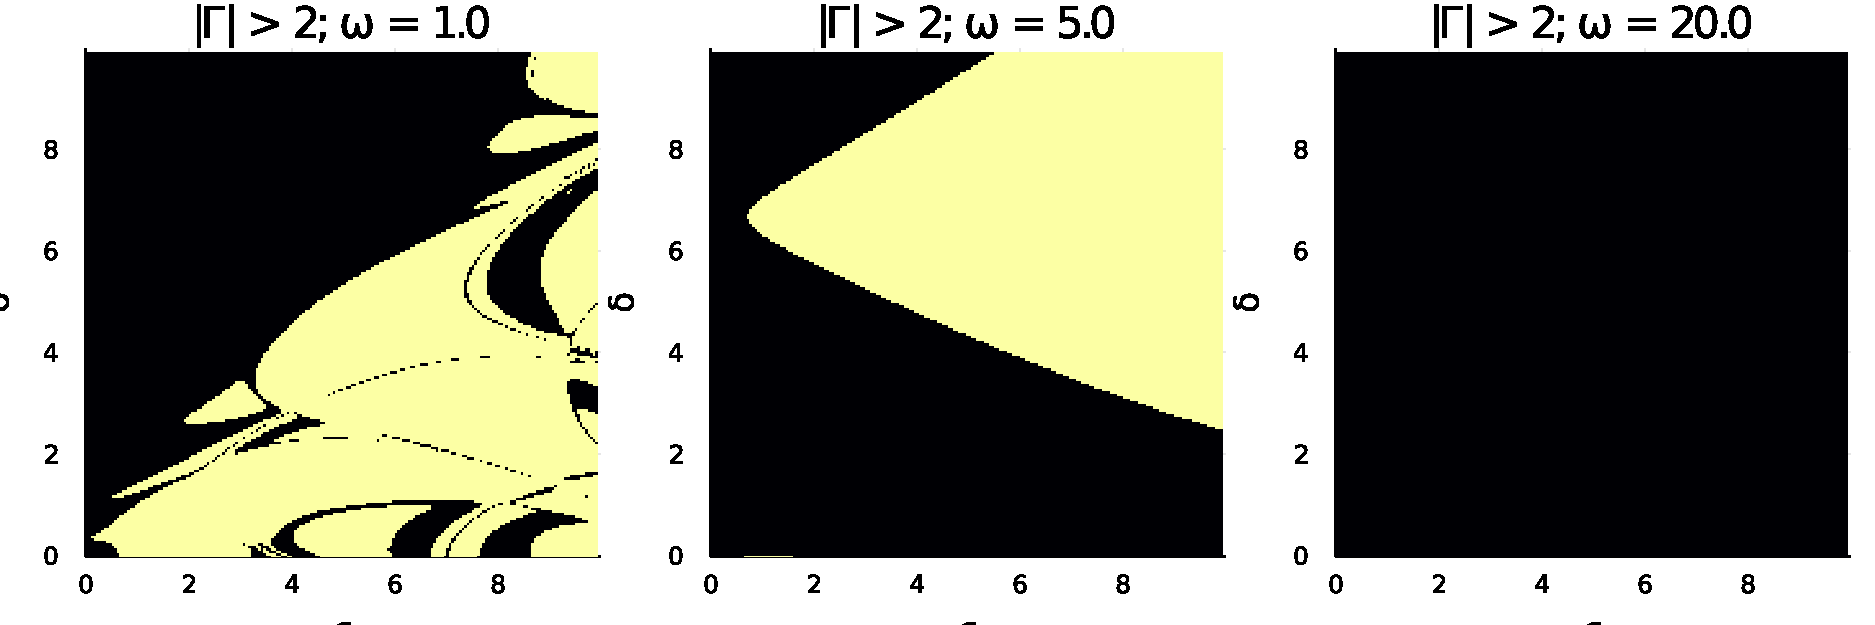
\includegraphics[width=0.9\textwidth]{../hw/figs/hw-7-exer-Floquet-binary.pdf}
     \end{subfigure}
     \hfill
     \caption{Visualizing the Floquet discriminant for $(\delta, \epsilon) \in [0, 10] \times [0, 10]$. We see for larger values of $\omega$ the pendulum is stablized.}
     \label{fig:floquet-heat}
\end{figure}

\end{sol}
\end{document}
